\documentclass[12pt, titlepage]{article}

\usepackage{booktabs}
\usepackage{tabularx}
\usepackage{graphicx}
\usepackage{hyperref}
\hypersetup{
    colorlinks,
    citecolor=black,
    filecolor=black,
    linkcolor=red,
    urlcolor=blue
}
\usepackage[round]{natbib}

\title{SIMS: User Guide}

\author{Team \#33, 'Sick Ideas'
		\\ Nathan Coit -- 400022342
		\\ Lucas Shanks -- 400029943
		\\ Cameron Van Ravens -- 400020215
}

\date{December 6, 2017}


\begin{document}

\maketitle

\pagenumbering{roman}



\pagenumbering{arabic}

\section{Overview}
This document provides a user walk through on using the basic functionality of the Synergy Inventory Management System (SIMS). Creating a company, adding items to inventory, tagging items, importing items, and editing account information, taking inventory snapshots, creating new employee accounts and changing company permissions are all covered in this document.


\section{Login Page}
To begin, access the SIMS login page at \href{https://synergyims.me}{https://synergyims.me}. From here, unless you are a returning user, you must create an account. Click the Create a company! link at the bottom of right of the box. This will redirect you to the registration page.
\begin{figure}[h]
\centering
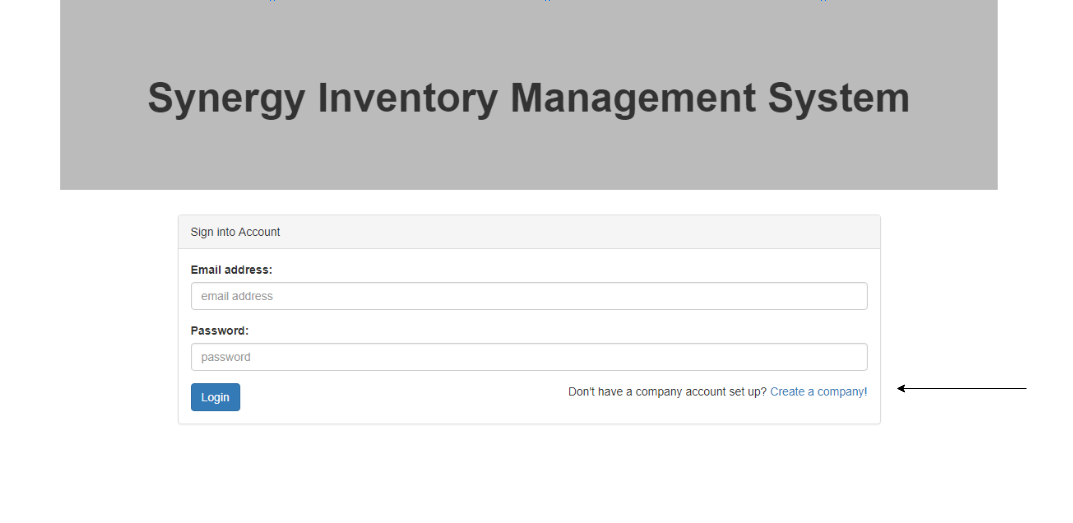
\includegraphics[width=\linewidth]{sims1.PNG}
\caption{Login Page}
\label{fig:figure1}
\end{figure}


\section{Registration Page}
At the registration page, you must fill all fields with the required information and follow directions shown on the screen. After hitting Submit, if no error is displayed, you will be redirected to the home page. If an error occurs such as the email is already in use, please follow the directions on the screen and change the required fields before clicking the submit button again.

\begin{figure}[h]
\centering
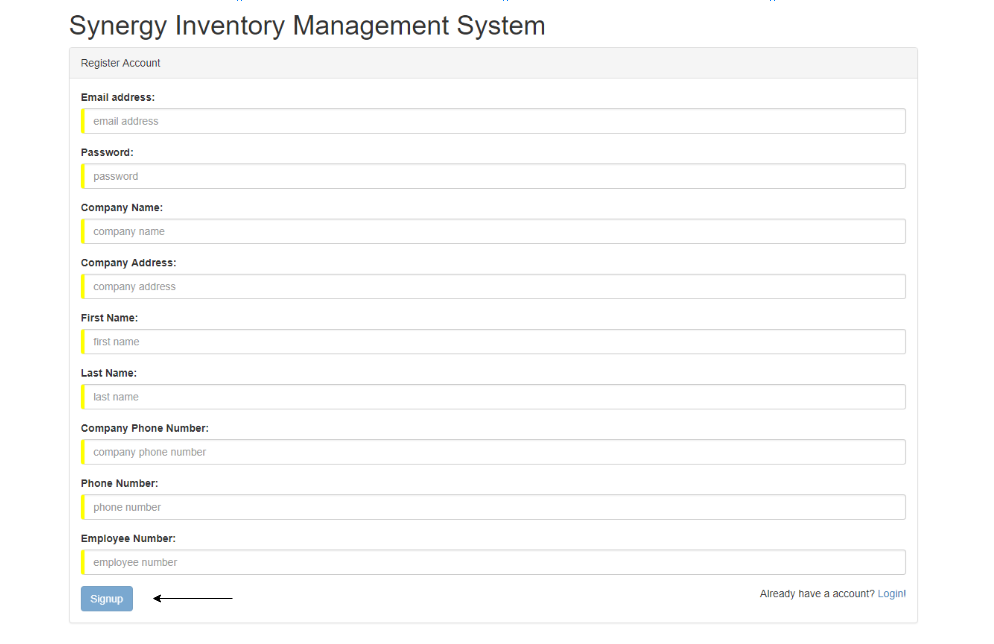
\includegraphics[width=\linewidth]{sims2.PNG}
\caption{Registration Page}
\label{fig:figure2}
\end{figure}

\section{Home Page}
At the home page, there are many options to choose from. You can find your company name located on the top-left side of the screen and a navigation bar located directly under the company name. Here, you will find the option to manage inventory, warehouses, brands, categories, company info, account info, or users profile information.\\

A secure logout button is located at the bottom of the navigation bar.To the right of the screen, various graphs and user inventory information is located and can be populated after user inventory information is uploaded and a \hyperref[sec:snapshot]{inventory snapshot} is created.
\begin{figure}[h]
\centering
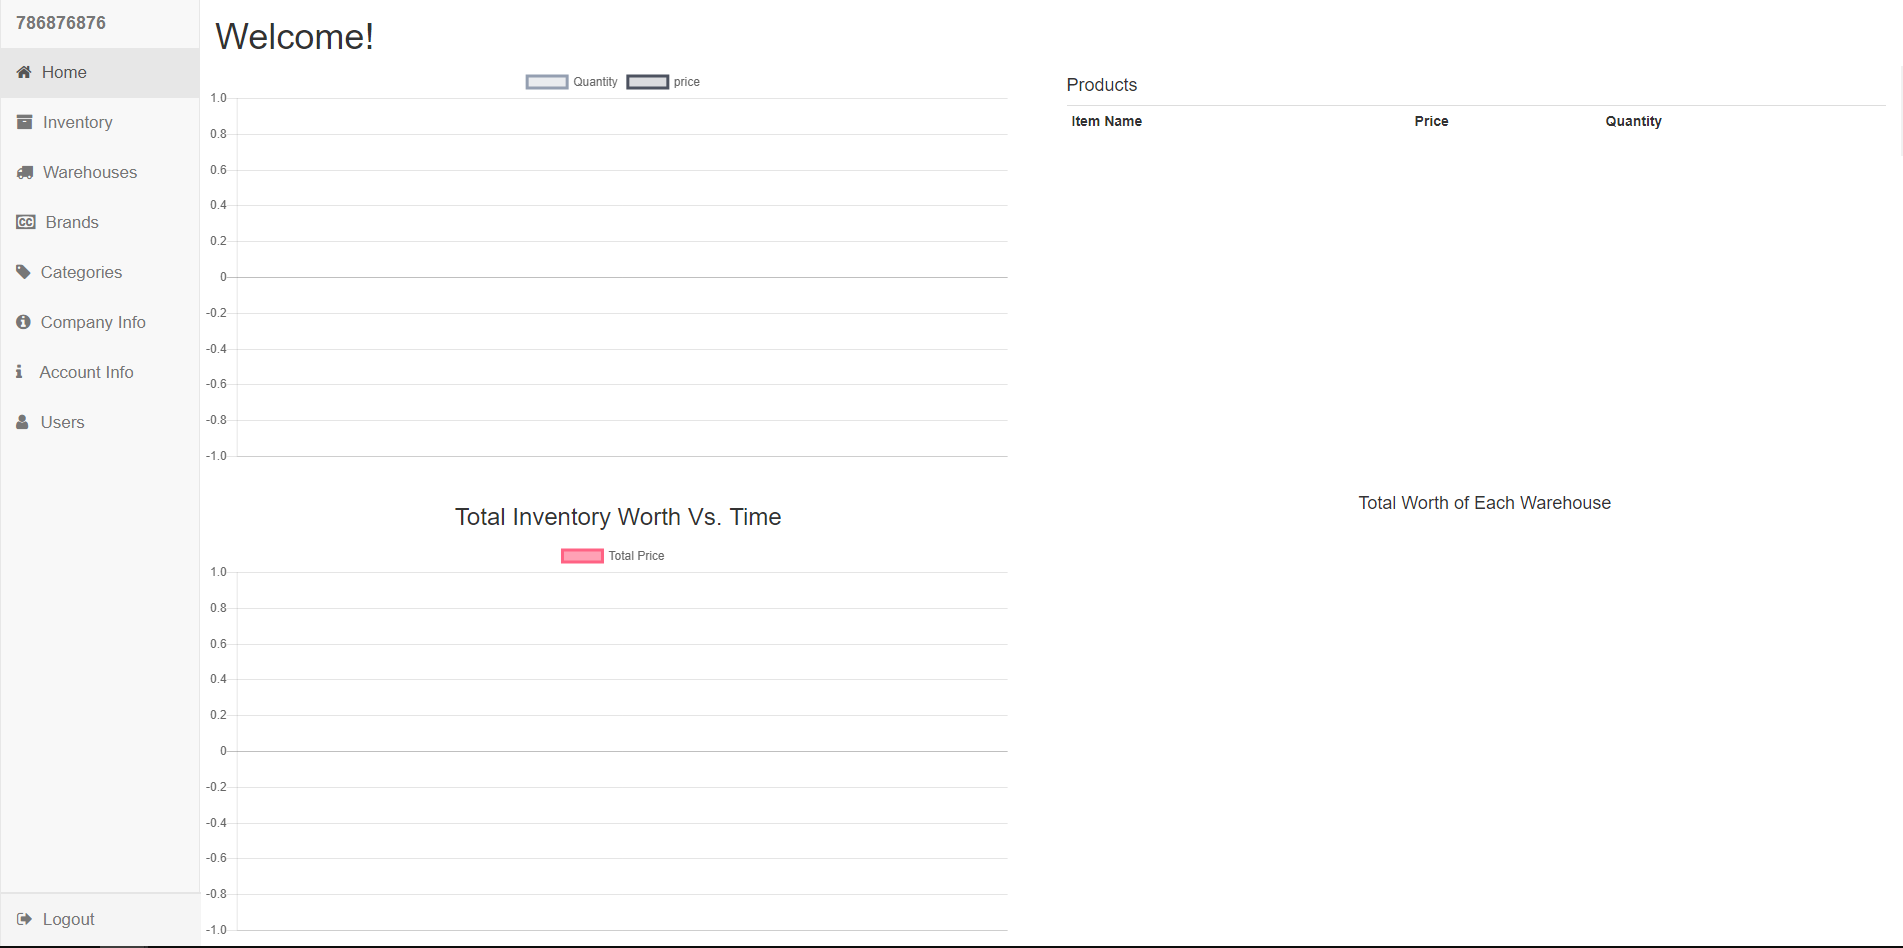
\includegraphics[width=\linewidth]{sims3.PNG}
\caption{Home Page}
\label{fig:figure3}
\end{figure}

\section{Inventory Page}
The inventory page is how you can keep track of the total inventory of a product in your company. At the top left, there is a search option to find specific items or items that begin with certain letters and a page limit option to set the number of items per page. On the top right, there is an option to import a csv. More information can be found in \hyperref[sec:csv]{Uploading a csv}. There is also the option to add an item to the inventory database. Please refer to \hyperref[sec:createitem]{Creating an item} for a detailed guide on adding an item to your inventory.\\

Finally, the headers of each column can be click to sort the column either alphabetically or by greatest value. The header can be clicked again to sort the rows reverse alphabetically or by lowest value. There are also options to edit an item or delete an item both found on the same row as the desired item by a wrench icon and a garbage bin icon respectively.
\begin{figure}[h]
\centering
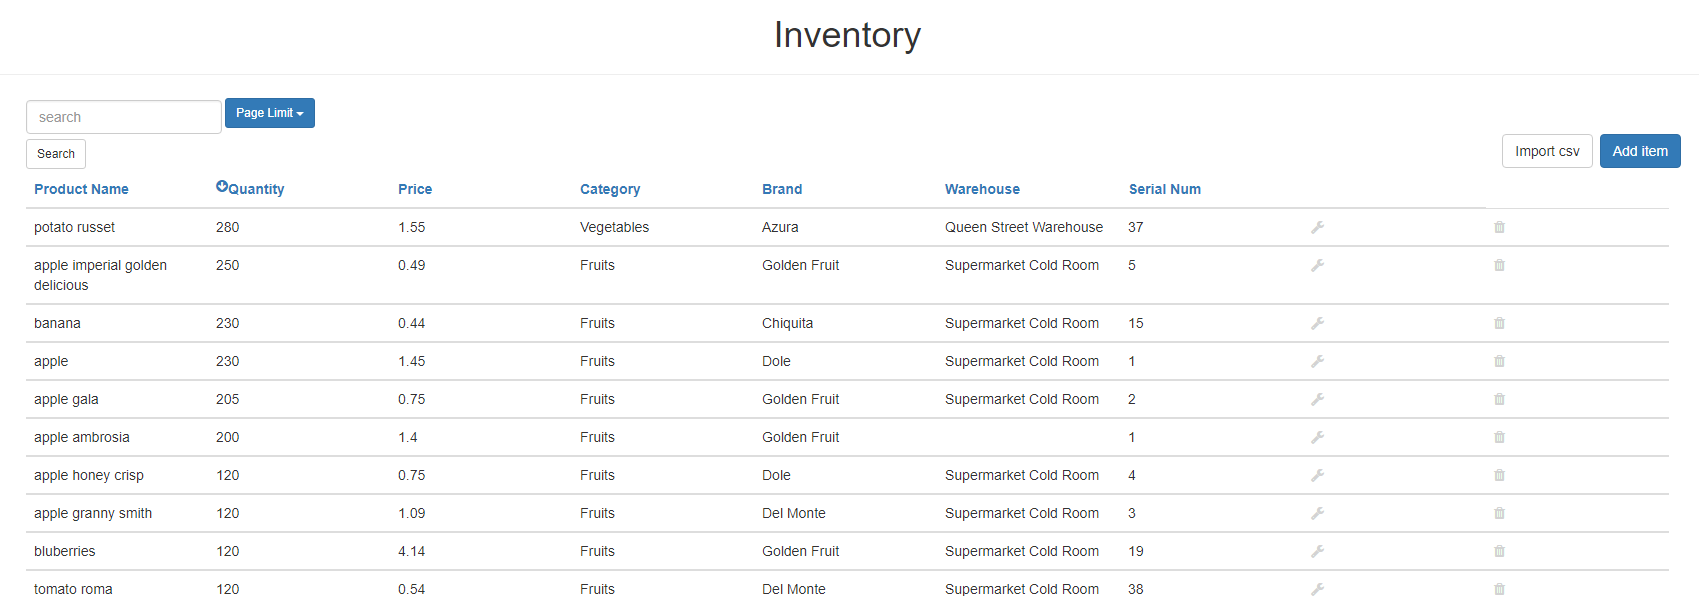
\includegraphics[width=\linewidth]{sims5.PNG}
\caption{Inventory Page. Quantity has been selected to sort the rows by greatest quantity of item in the database.}
\label{fig:figure4}
\end{figure}
\newpage

\section{Creating an item}
\label{sec:createitem}
This section will explain how to add an item to your inventory. On the inventory page, after selecting the add item button, a modal will appear prompting you for the required information about the product. Here after providing the item name and any description, tags can be assigned to the item including Brands, Categories, or Warehouses that the product belongs to. \\

These options are available to help you sort your inventory and keep track of items with more than just the product name. Finally, price, quantity, and serial number can be added for the product before adding the new item to your inventory.

\begin{figure}[h]
\centering
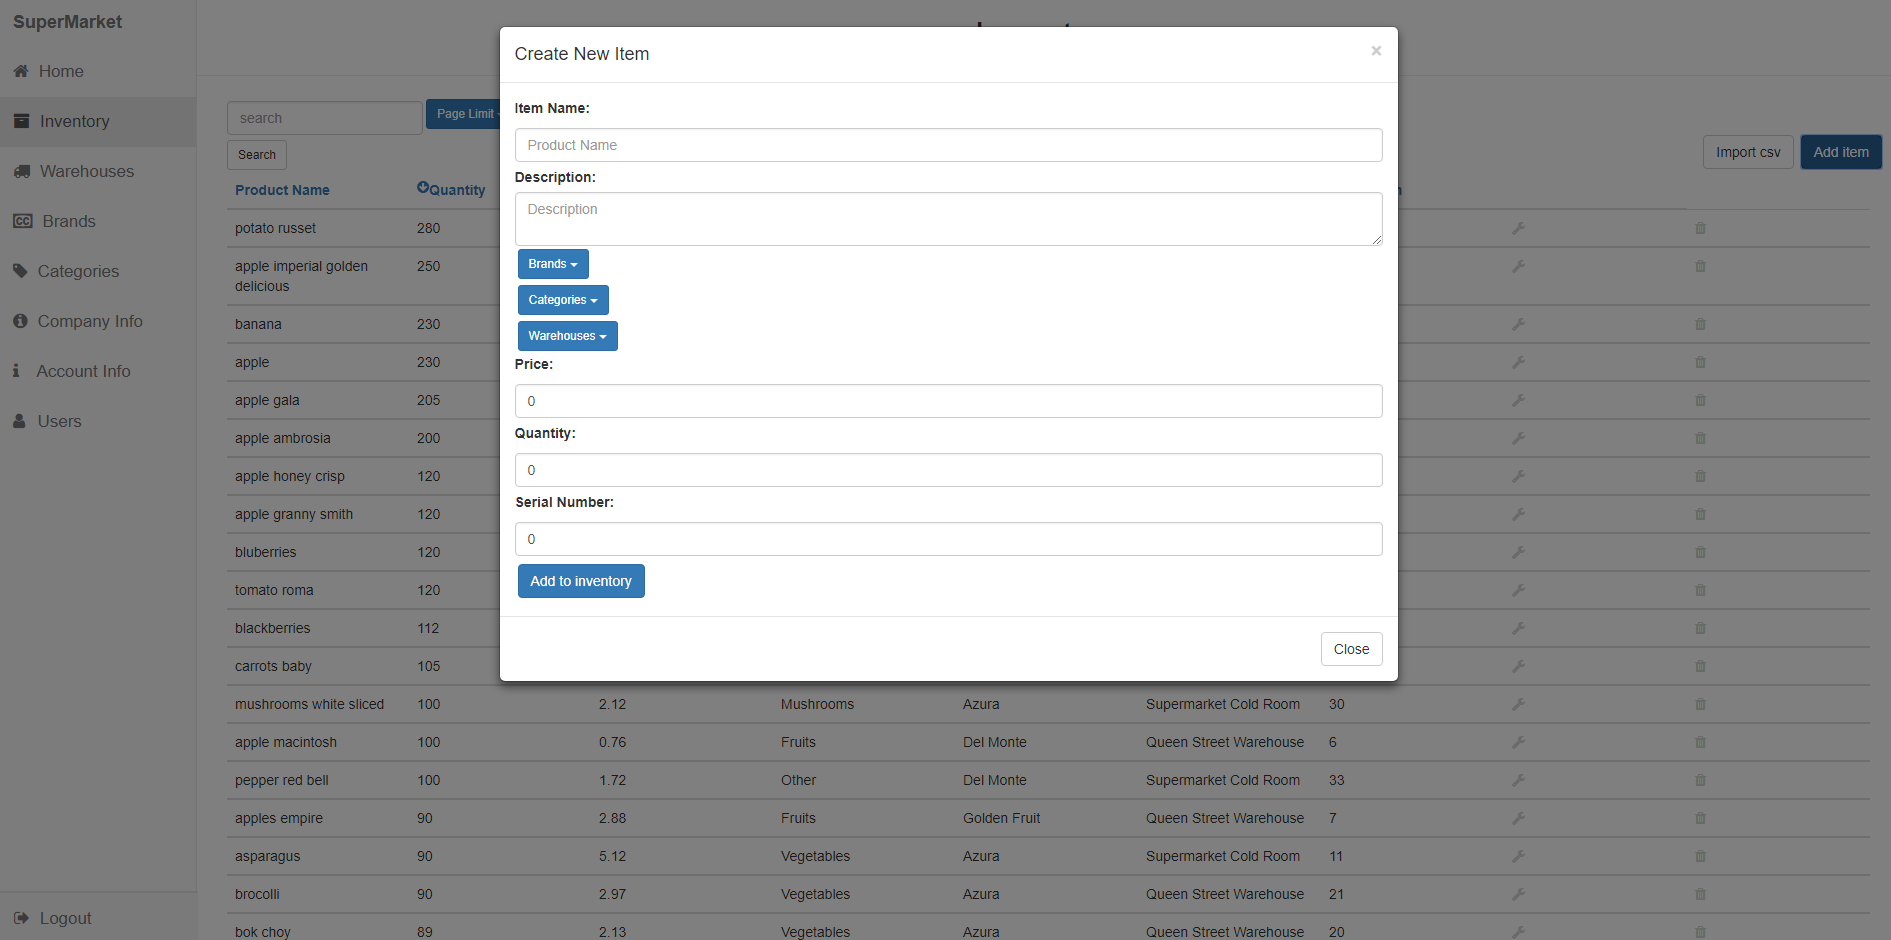
\includegraphics[width=\linewidth]{sims6.PNG}
\caption{Add item}
\label{fig:figure4}
\end{figure}

\section{Warehouse, Brands, and Categories Page}
\label{sec:warehouse}
The following three pages are all selectable on the left navigation bar and all allow you to add different tags to the products in your inventory. Here, you will find options to both Add a new warehouse, brand, or category, as well as delete already set options as well.

\section{Company Info}
\label{sec:companyinfo}
Here you will find information about the company including the ability to edit the company name, address or phone number. There is also the option to your company. This page is also restricted, meaning the page is only accessible by the owner of the company (the user that created the company account). Here, options are also available to change permissions for the users. Here, an owner can change what access an Admin account has to a specific page, as well as change the level of access a regular user has to a specific page. These options can be toggled by selecting the green true/false options.

\begin{figure}[h]
\centering
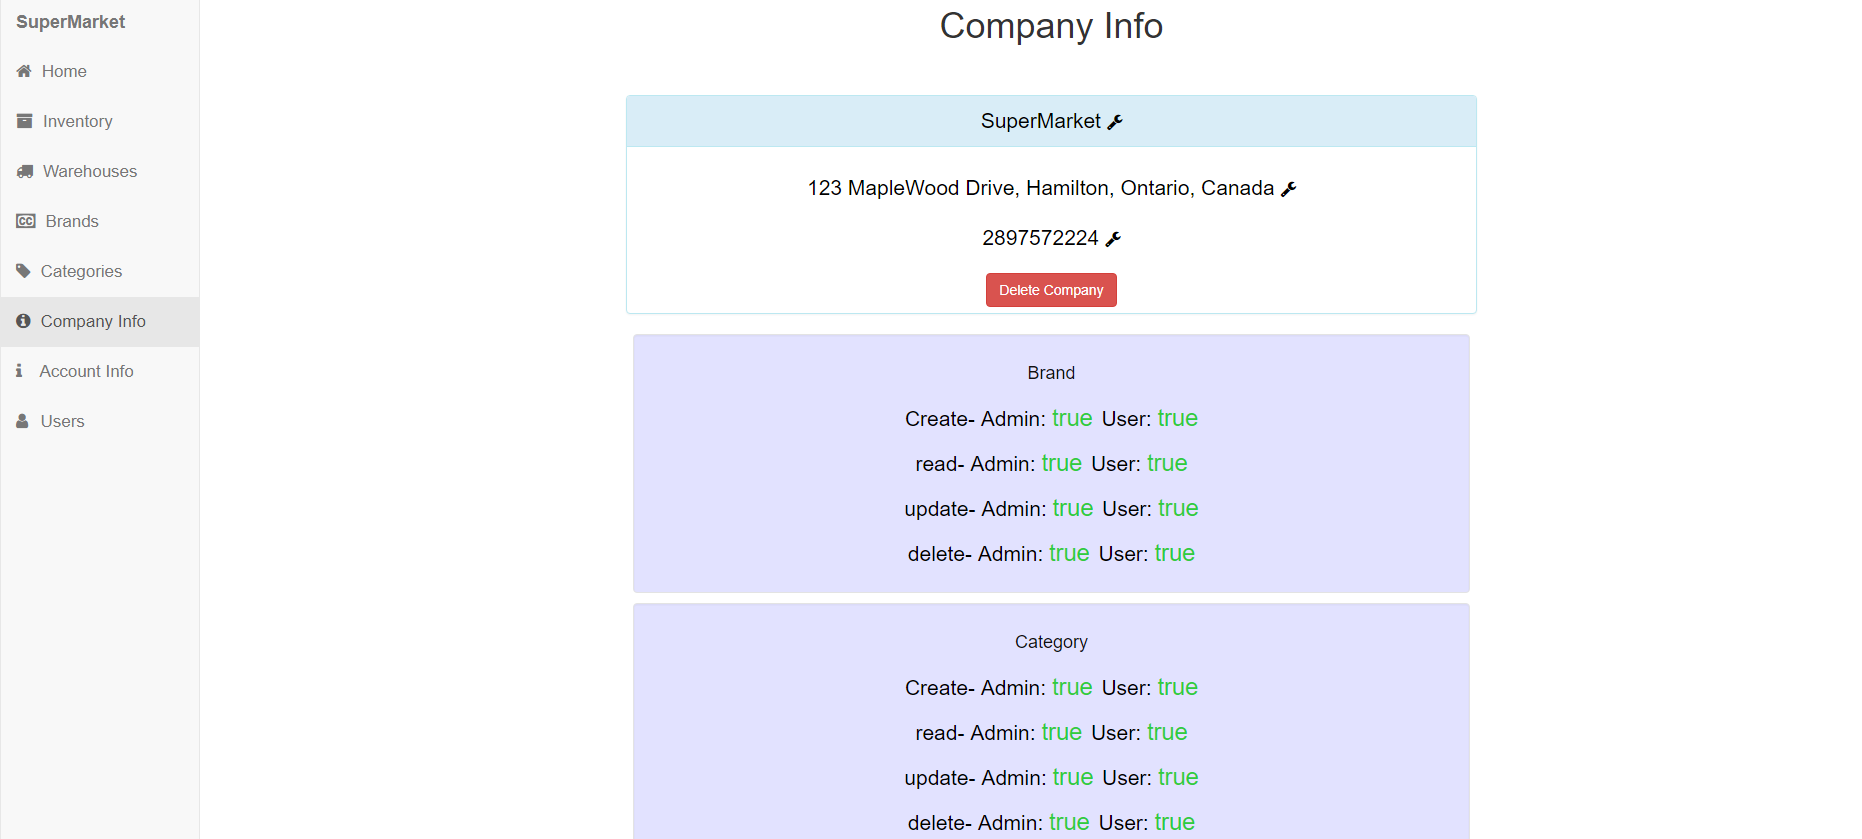
\includegraphics[width=\linewidth]{sims7.PNG}
\caption{Company Info}
\label{fig:figure4}
\end{figure}

\section{Account Info}
\label{sec:info}
Here you will find information about the user account with the ability to edit user information including first name, last name, email, phone number, employee number, and password.

\section{Users Page}
\label{sec:info}
Here you will find information about all user accounts registered with the company. Here, you will find the option to add a new user, as well as edit or delete current users. This page is designed to allow employees to have accounts created for them with limited access to restricted pages. Here, a user may be created with the Add User button and granted an access level of either admin or user. Access levels for these account types can be changed in the \hyperref[sec:companyinfo]{Company info page}.

\section{Uploading a csv}
\label{sec:csv}
In this section, you may upload your own formatted csv to populate or edit your products page instead of manually changing item information. Here, a csv must be uploaded with properly formatted fields following the style:
item\_name,description,price,quantity,serial\_num\\
a,b,0,0,0\\
c,d,0,0,0\\
...\\

\section{Creating an inventory snapshot}
\label{sec:snapshot}
To create an inventory snapshot to show the graphs on the Home Page with your inventory data, you must first create an inventory snapshot. Navigate to the inventory page. At the bottom right you will find an option labeled Create Snapshot. From here, a snapshot will be created for all items currently in the database.\\

Now navigating to the Homepage will reveal 3 graphs. The line graph has clickable inventory items that display the change in quantity between snapshots, the bar-graph compares the total items in the inventory between snapshots, and the pie chart represents the total worth of all items in each warehouse.

\begin{figure}[h]
\centering
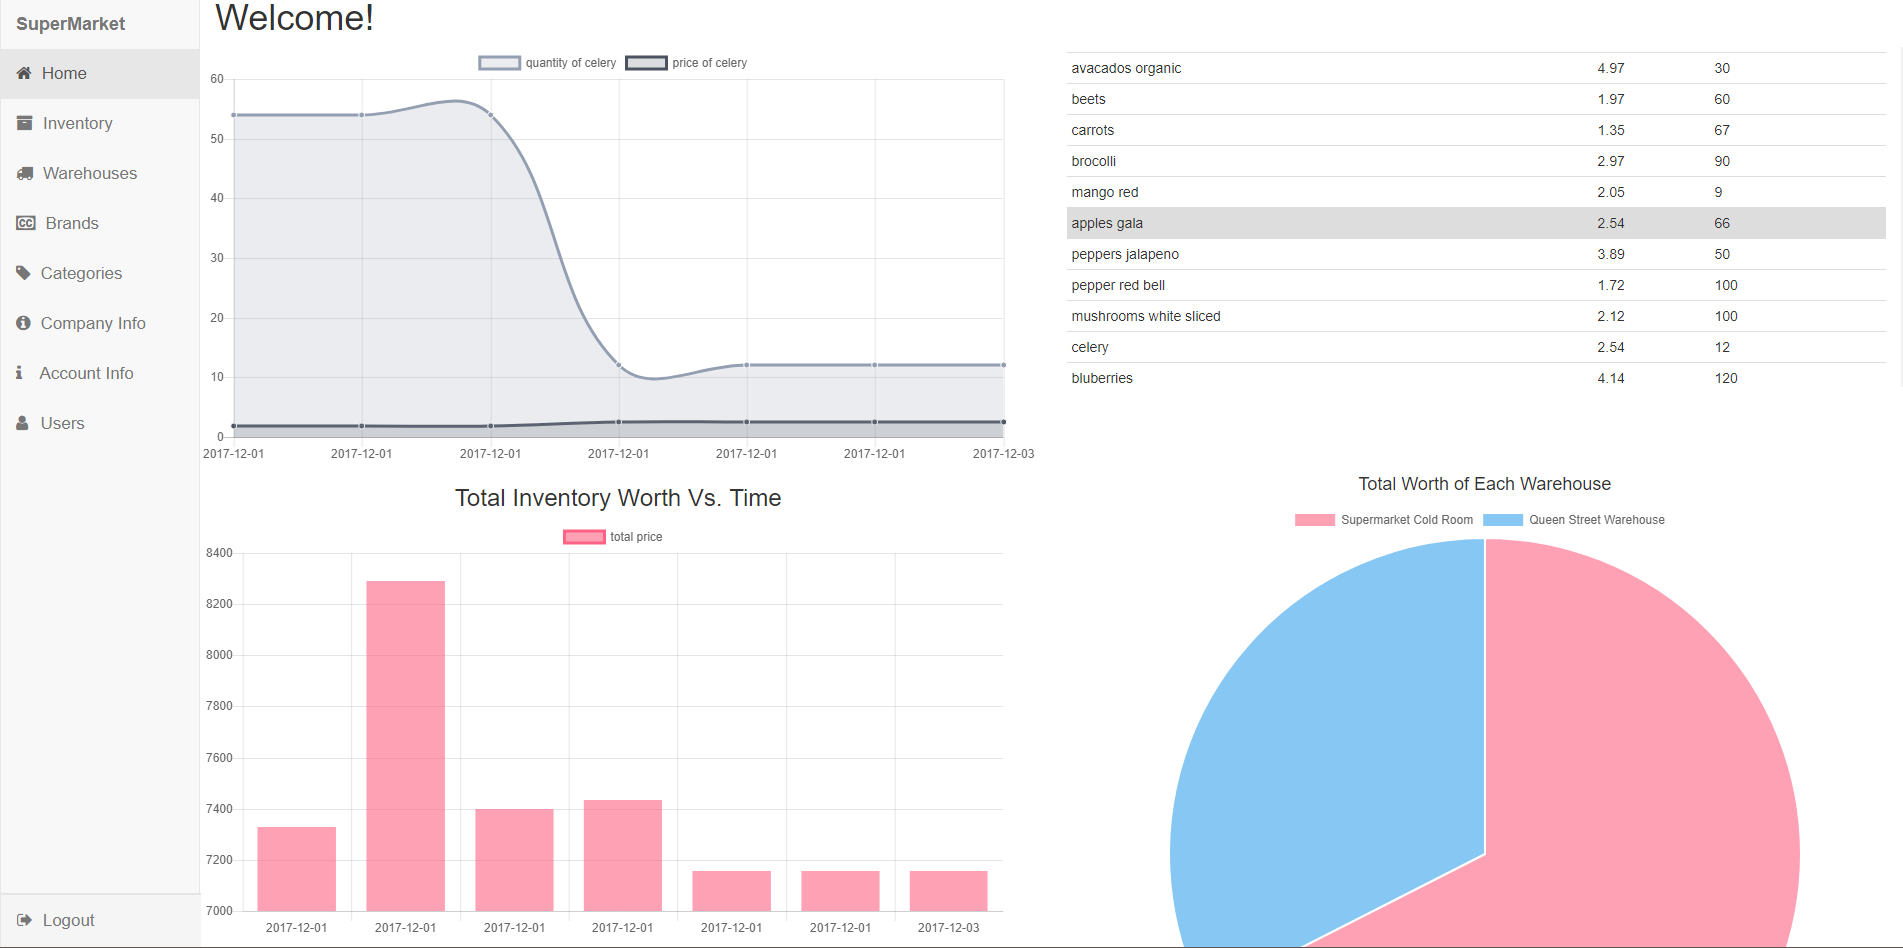
\includegraphics[width=\linewidth]{sims4.PNG}
\caption{Inventory Snapshot}
\label{fig:figure5}
\end{figure}

\end{document}
